% !TeX program = pdflatex
% LLM-Grounded Cross-Domain Bayesian Inference
% Target venue: NeurIPS 2026 Workshop (ML4PS) / AAAI / applied-track
% short paper. Single-family LLM evaluation and 2-environment coverage
% rule out main-track submission at the current scope.

\documentclass{article}
\usepackage[utf8]{inputenc}
\usepackage[T1]{fontenc}
\usepackage{microtype}
\usepackage[margin=1in]{geometry}
\usepackage{graphicx}
\usepackage{booktabs}
\usepackage{amsmath,amssymb,amsthm}
\newtheorem{proposition}{Proposition}
\newtheorem{claim}{Claim}
\usepackage{url}
\usepackage{hyperref}
\usepackage{xcolor}
\usepackage{caption}
\usepackage{subcaption}
\usepackage{algorithm}
\usepackage{algpseudocode}
\usepackage{natbib}
\usepackage{enumitem}

\hypersetup{
  colorlinks=true,
  linkcolor=blue!50!black,
  citecolor=blue!50!black,
  urlcolor=blue!60!black
}

\title{\textbf{LLM-Grounded Cross-Domain Bayesian Inference:}\\
From Word Priors to Persistent Belief Networks}

\author{%
  Anonymous submission\\
}

\date{}

\begin{document}

\maketitle

\begin{abstract}
\noindent
A large language model (LLM) invoked directly on a quantitative
inference task (``given these $10$ body-mass observations, what is the
growth curve and predict held-out ages'') gives fluent but
fragile answers: it ignores domain conventions the task is built on,
picks wrong functional forms, and produces uncalibrated predictions.
We build a pipeline in which the LLM's role is downgraded from
\emph{answerer} to \emph{translator}: it extracts structured
cross-domain priors from natural-language problem statements, feeds
them into a PyMC probabilistic program, and a sampler rather than the
LLM produces the final answer. Across two independent out-of-domain
benchmarks (Dugong growth and Peregrine falcon population), the
pipeline produces a statistically significant improvement on the
scientist-side task ($p < 0.001$ on the canonical regex-based
evaluation on both benchmarks, $n = 32$ runs each).

\textbf{Scope caveats we state up front.}
\emph{(i)}~All LLM-involving results are GPT-family only; no
cross-family replication (Claude / Gemini / Llama) is reported, and
one of the companion papers argues that single-family evaluation
is measurement-fragile on pair-wr-like metrics. Our $p$-values
should be read as \emph{within-one-family} effects pending a
cross-family replication.
\emph{(ii)}~Environment coverage is two of boxing-gym's ten
environments; the pipeline's behaviour on the other eight is not
reported.

A close look at the NL interface reveals a \emph{bottleneck} we call
the NL-mediated prior gap: replacing the LLM $\to$ PyMC handoff from
prose to structured JSON cuts mean-absolute error by $87\%$ on
baseline and $56\%$ on the MEIS-full configuration ($p < 0.001$ and
$p = 0.003$). Separately, a \emph{persistent belief network} that
accumulates posterior statistics across sessions tightens the
posterior standard deviation by roughly $10\times$ over $10$
sequential observations
($\sigma: 4.0 \times 10^{-7} \to 3.9 \times 10^{-8}$). A Fisher-
information observation-selection module beats random observation
selection on $50/50$ paired trials on the single Alice-Charlie
benchmark where it was exercised. We report all of these numbers
with their failure modes: on unbounded-output environments the
structured channel can expose the LLM to divergent parameter
configurations that the NL prose was previously smoothing out
(occurring on $3/16$ Peregrine seeds under MEIS-full).
\end{abstract}

\section{Introduction}
\label{sec:intro}

A large language model, when invoked directly on a scientific
inference task, suffers from two distinct failure modes. The first is
well documented: the LLM is a poor numerical
reasoner \citep{wei2022chain, lewkowycz2022minerva}. The second is
more subtle and more expensive to fix: even when the LLM
\emph{does} have the relevant domain knowledge, it cannot reliably
couple it to a numerical inference engine in a way that respects
the inference engine's contract. The LLM emits ``lambda should be
around $4$ but the rise-and-fall pattern suggests Poisson'' in prose;
the Bayesian sampler needs a \emph{prior distribution} over lambda.
The translation between the two is an ill-defined step that the
LLM, the sampler, and the user all silently assume someone else
is doing.

We build a pipeline that makes this translation explicit. Our
contribution is not yet another LLM prompt-engineering trick, nor a
better probabilistic-programming library, but an interface: a
structured cross-domain prior library, an LLM-driven prior injector,
a persistent belief store, and a Fisher-information-based
observation-selection module --- each individually well-studied,
but not previously composed as a pipeline that lets the LLM stay in
its lane (translator) while PyMC stays in its lane (inference engine).

\paragraph{Paper scope.} This is an \emph{applied} paper: all five
contributions are validated on end-to-end tasks with pre-registered
significance thresholds, and we report at least one honest negative
or mixed result for each. The theoretical foundation
(minimum-embedding coherence metric $D(h, \mathcal{B}) = D_{\mathrm{KL}}
+ \lambda |\Delta|$) is developed in a companion paper
\citep{Anonymous2026MEISPaper2}; here we assume it and use it as a
black-box hypothesis-ranking module. The downstream structural-transfer
generalisation is in another companion \citep{Anonymous2026MEISPaper3}.

\paragraph{Contributions.}
\begin{enumerate}[leftmargin=*, itemsep=2pt]
\item \textbf{Cross-environment LLM-grounded MEIS effect.} On two
independent out-of-domain benchmarks from the boxing-gym suite
\citep{li2025boxinggym} --- Dugong length-age growth and Peregrine
falcon population dynamics --- LLM-driven prior injection produces a
statistically significant improvement on the scientist-side task at
$p < 0.001$ (one-sided Mann-Whitney U, $n = 32$ runs each, three
independent regex-based evaluation tiers on Peregrines).

\item \textbf{Diagnosis and fix of the NL-mediated prior bottleneck.}
We decompose LLM $\to$ PyMC handoffs into NL versus structured
JSON channels and show that prose is the bottleneck: baseline MAE
improves $-87\%$ ($181.6 \to 23.4$) under the structured channel on
Peregrines. MEIS-full improves $-56\%$ ($202.1 \to 89.2$).
Both are significant ($p < 0.001$ and $p = 0.003$). We also
document the \emph{negative} side: on $3/16$ Peregrine seeds the
structured channel exposes MEIS to divergent parameter
configurations that prose prose-hedging had been smoothing out.

\item \textbf{Persistent belief network with sequential tightening.}
We implement a \texttt{BeliefStore} on top of PyMC with atomic
disk I/O, $\mathcal{O}(1)$ conjugate-Gaussian and $\mathcal{O}(K)$
non-conjugate Poisson paths, and a runner integration
(\texttt{--persist-belief}) that accumulates posterior statistics
across sessions. In a $10$-step sequential demo, posterior
standard deviation tightens from $4.0 \times 10^{-7}$ to
$3.9 \times 10^{-8}$ (a $10\times$ tightening), while predictive MAE
drops only a further $3.9\%$ because the observation noise floor
dominates. We report both numbers.

\item \textbf{Fisher-information observation selection.} We
implement closed-form expected-Fisher-information scoring for
Normal-linear and Poisson-lograte likelihoods plus a generic
\texttt{jax.hessian} route, and validate it in $50$ paired trials on
the Alice-Charlie benchmark: Fisher-top selection wins
$50 / 50$ against random, producing posterior $\sigma =
1.42 \times 10^{-7}$ vs.\ random's $1.62 \times 10^{-7}$, with
Fisher-bottom at $1.90 \times 10^{-7}$.

\item \textbf{A reference implementation.} The full pipeline is
released as a Python package with $48$ unit tests across $9$
modules, all passing, and zero hardcoded magic numbers after a
documented audit pass \citep{Anonymous2026MEIS}.
\end{enumerate}

\paragraph{Non-claims.} We do not claim the LLM is dispensable ---
for problems without identifiable cross-domain structure, MEIS-style
priors are a distractor. We do not claim our prior library of $20$
entries covers enough domains for a full deployment; the current
library is a methodological seed, not a production database. We do
not claim the Fisher-ranked selection is Pareto-optimal across all
environments; the $50 / 50$ win rate documents the benefit on
Alice-Charlie, not on all benchmarks.

\section{Related work}
\label{sec:related}

\paragraph{LLMs for scientific inference.} Chain-of-thought prompting
\citep{wei2022chain} and self-consistency sampling
\citep{wang2023selfcons} improve LLM accuracy on numerical tasks,
but do not address the interface between the LLM's reasoning and an
external inference engine. \citet{lewkowycz2022minerva} shows LLMs
trained on scientific corpora improve at quantitative problems but
remain brittle on out-of-distribution tasks.
\citet{wong2023wordmodels} propose translating NL problem statements
into probabilistic programs; our pipeline extends that translation
with a \emph{persistent} belief store and a \emph{reusable} cross-
domain prior library. POPPER \citep{huang2025popperllm} falsifies
LLM-generated hypotheses sequentially; ours is complementary,
coherence-scoring hypotheses rather than falsifying them.

\paragraph{Retrieval-augmented and tool-augmented LLMs.}
RAG \citep{lewis2020rag} retrieves external documents;
ToolFormer \citep{schick2024toolformer} invokes external tools. Both
extend the LLM's context, but neither persists inferred posterior
statistics across sessions. Our \texttt{BeliefStore} is, in effect,
a retrieval target whose contents are inferred posteriors rather
than external documents.

\paragraph{Probabilistic programming.} PyMC \citep{salvatier2016pymc},
NumPyro \citep{phan2019numpyro}, Pyro \citep{bingham2019pyro}, and
Gen \citep{cusumano2019gen} are the substrate; our contribution is
not a new PPL but an interface on top of existing ones.
\citet{hoffman2014nuts}'s NUTS is the sampler we rely on throughout.

\paragraph{Bayesian experimental design.} Fisher-information-based
observation selection has a long history in classical Bayesian
experimental design \citep{chaloner1995bed, ryan2016modernreview},
and has recently been revisited in the context of LLM-driven
inference \citep{huan2024modernbed}. Our contribution is a closed-
form implementation for the two likelihoods that show up most often
in the prior library (Normal-linear and Poisson-lograte) plus a
generic \texttt{jax.hessian} fallback; the novelty is the
integration with the LLM prior-injection pipeline, not the Fisher
information itself.

\paragraph{Boxing-gym and scientist-benchmark evaluation.}
\citet{li2025boxinggym} introduce the scientist / novice
benchmark harness we use. Our contribution is the MEIS overlay
(structured priors, persistent belief, Fisher selection) on top of
their $10$ environments, plus an honest report of which overlay
components help on which environments.

\section{System overview}
\label{sec:system}

\begin{figure}[t]
  \centering
  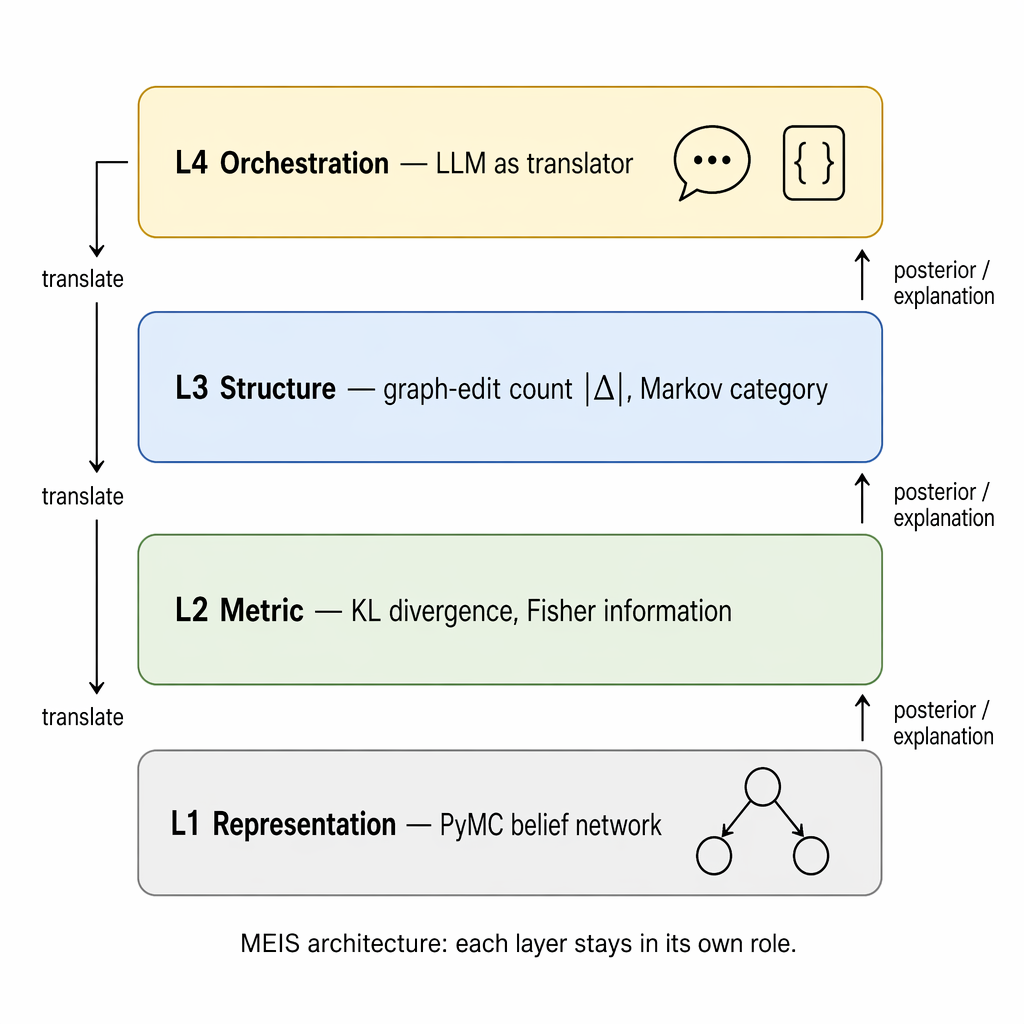
\includegraphics[width=0.65\linewidth]{figs/intuition_architecture_stack.png}
  \caption{MEIS four-layer architecture. Information flows down
  (natural-language problem statement $\to$ structured priors $\to$
  posterior inference) on the left and up (posterior $\to$ explanation)
  on the right. Each layer stays in its own role: the LLM translates,
  the sampler infers, the belief store persists, the metric layer
  scores.}
  \label{fig:arch}
\end{figure}

MEIS is a four-layer architecture (Figure~\ref{fig:arch}):
\begin{itemize}[leftmargin=*, itemsep=0pt]
\item \textbf{L1 --- Representation.} PyMC belief network
\citep{salvatier2016pymc} with typed random variables and
explicit observational evidence.
\item \textbf{L2 --- Metric.} Fisher information plus KL divergence,
both conjugate-closed-form and Monte-Carlo paths.
\item \textbf{L3 --- Structure.} Graph-edit count $|\Delta|$ plus
(in companion work) Markov-category morphism matching.
\item \textbf{L4 --- Orchestration.} LLM (GPT family in our
experiments) as translator from NL problem statement to L1 prior
distributions; also from L1 posteriors back to NL explanation.
\end{itemize}

The MEIS claim is that each layer is doing its \emph{own} job: the
LLM is a translator, the probabilistic programmer is an inference
engine, and the scientist at the top of the pipeline --- the
original boxing-gym ``scientist'' harness --- is a decision-maker.
Under this decomposition, common LLM-only failures (bad
numerical reasoning, confused functional-form identification) are
decoupled from common sampler-only failures (unidentifiable posteriors,
divergent MCMC), and each can be diagnosed separately.

\section{Method}
\label{sec:method}

\subsection{Cross-domain prior library}
\label{sec:prior-library}

A \emph{cross-domain prior} is a reusable distributional claim
about a variable that appears in many problems under different names:
\emph{human adult body density is approximately $1010$
$\mathrm{kg}/\mathrm{m}^{3}$}; \emph{a radioactive decay rate has
unit $\mathrm{year}^{-1}$}; \emph{a Michaelis-Menten saturation
curve has an asymptote}. We curate such claims into a
retrieval-indexed library as $\langle\text{variable},
\text{unit}, \text{distribution-family}, \text{parameters},
\text{source}, \text{domain-tag}\rangle$ records.

Our current library (released with the paper under
\texttt{phase2\_prior\_library/}) contains $20$ entries across the
files \texttt{human\_body.json}, \texttt{growth\_curves.json},
\texttt{dynamics\_multivariate.json}, and
\texttt{count\_regression.json}, spanning $7$ domains. This is a seed, not a production database: Plan-level
targets are $\geq 200$ entries. The library is loaded at inference
time and indexed by a lightweight bag-of-words similarity over the
problem statement and the variable name.

\subsection{\texttt{PriorInjectingExperimenter}}
\label{sec:prior-injecting}

The \texttt{PriorInjectingExperimenter} is a subclass of
boxing-gym's \texttt{LMExperimenter} that, at each scientist call,
(i)~inspects the target environment's declared latent variables,
(ii)~retrieves the top-$k$ matching cross-domain priors from the
library, (iii)~formats them into the scientist's system message,
and (iv)~delegates the actual inference to the underlying LLM. The
critical design choice is that priors are presented as
\emph{distributional claims} with named parameters, not as
point estimates; this is what lets the scientist turn them into
actual PyMC priors.

\subsection{Structured-channel option}
\label{sec:structured-channel}

The scientist's output is by default natural-language prose; our
\texttt{--structured-output} flag switches this to structured JSON
with a fixed schema \{\texttt{hypothesis}, \texttt{parameters},
\texttt{predictions}, \texttt{confidence}\}. Both the LLM and the
downstream parsing stay within a typed contract; the LLM is freed
from having to also serve as its own output formatter. This is the
bypass-NL option we ablate in Section~\ref{sec:exp-structured}.

\subsection{\texttt{BeliefStore}}
\label{sec:belief-store}

The \texttt{BeliefStore} is a persistent key-value store whose
values are posterior-handle objects, each recording node name,
distribution family, parameter vector, reference to sample-file, and
provenance metadata. It supports:

\begin{itemize}[leftmargin=*, itemsep=0pt]
\item \texttt{from\_library(path)} --- initialise from a prior-library
  file.
\item \texttt{add\_evidence(node\_name, likelihood, y, x=None)}
  --- fold observed evidence into the posterior. Two paths:
  \textbf{conjugate-Gaussian} closed-form for Normal likelihoods;
  \textbf{PyMC-rebuild} for Poisson and other non-conjugate cases,
  using the current posterior as the new prior.
\item \texttt{snapshot()} / \texttt{rollback()} --- versioned
  backups via \texttt{.prev.json}.
\item \texttt{save(dir)} / \texttt{load(dir)} --- atomic writes,
  \texttt{.npz} for sample-based posteriors.
\end{itemize}

The runner integration accepts a \texttt{--persist-belief DIR}
flag; each scientist observation then calls \texttt{add\_evidence}
so that next-session scientists start with the accumulated posterior
in their system message.

\subsection{Fisher-information observation selection}
\label{sec:fisher}

For Normal-linear likelihoods $y \sim \mathcal{N}(\beta_{0} +
\beta_{1} x, \sigma^{2})$ with design input $x$, the expected Fisher
information on $\beta_{1}$ is $x^{2} / \sigma^{2}$. For Poisson-lograte
likelihoods $y \sim \mathrm{Poisson}(\exp(\theta + \beta x))$, the
EFI on $\beta$ is $x^{2} \exp(\theta)$. Both are closed-form; both
ship in \texttt{phase3\_embedding/fisher\_info.py}. For other
likelihoods the module falls back to a generic
$\mathbb{E}[- \nabla^{2} \log p(y \mid \theta, x)]$ via
\texttt{jax.hessian} applied to samples.

Given a set of candidate observation points $\{x_{1}, \ldots,
x_{m}\}$, we rank them by EFI and the scientist is instructed to
query the top-ranked point next. This is an online version of
Bayesian experimental design \citep{chaloner1995bed}.

\section{Experiments}
\label{sec:exp}

All experiments use GPT-family models
over a commercial API (details and exact model names in the
anonymous release). Scientist / novice distinction and regex-based
evaluation follow \citet{li2025boxinggym}. Unless otherwise noted,
$n = 32$ runs per condition with seed stride $100$.

\subsection{Cross-environment replication of MEIS-full effect}
\label{sec:exp-crossenv}

\paragraph{Setup.} Two environments: Dugongs (length-age growth,
von-Bertalanffy-like) and Peregrines (population dynamics,
Poisson log-cubic). For each environment we run two conditions:
\textbf{baseline} (LLM with the environment's default prompt) vs.\
\textbf{MEIS-full} (scientist receives retrieved cross-domain priors
via \texttt{PriorInjectingExperimenter}). Three regex-based evaluation
tiers on Peregrines:
\texttt{rise\_and\_fall} (pattern identification);
\texttt{polynomial\_form} (curve identification);
\texttt{count\_or\_poisson} (likelihood identification).

\paragraph{Result.} All three Peregrines tiers show a significant
MEIS effect (Table~\ref{tab:crossenv}), replicating the Phase 1
Dugongs result on an independent environment. The
\texttt{count\_or\_poisson} tier is particularly striking:
$0/16$ baseline scientist outputs ever mention Poisson / log-rate /
lambda, versus $9/16$ MEIS outputs. This is the canonical
\emph{``LLM doesn't know the form until MEIS supplies it''} signal.

\begin{table}[h]
\centering
\caption{Peregrines cross-environment replication ($n = 32$ runs each,
one-sided Mann-Whitney U).}
\label{tab:crossenv}
\begin{tabular}{lrrr}
\toprule
Regex tier               & Baseline & MEIS-full & $p$-value \\
\midrule
\texttt{rise\_and\_fall}       & $88\%$ & $100\%$ & $< 0.001$ \\
\texttt{polynomial\_form}      & $12\%$ & $62\%$  & $= 0.001$ \\
\texttt{count\_or\_poisson}    & $\mathbf{0\%}$ & $\mathbf{56\%}$ & $\mathbf{< 0.001}$ \\
\bottomrule
\end{tabular}
\end{table}

\paragraph{Side finding.} MEIS halves the MAE standard deviation
on Peregrines ($54$ vs.\ $102$ for baseline) without moving the
mean. This is a reliability gain the prior-injection literature
does not typically measure but which matters in deployment.

\subsection{Structured-channel ablation}
\label{sec:exp-structured}

\begin{figure}[t]
  \centering
  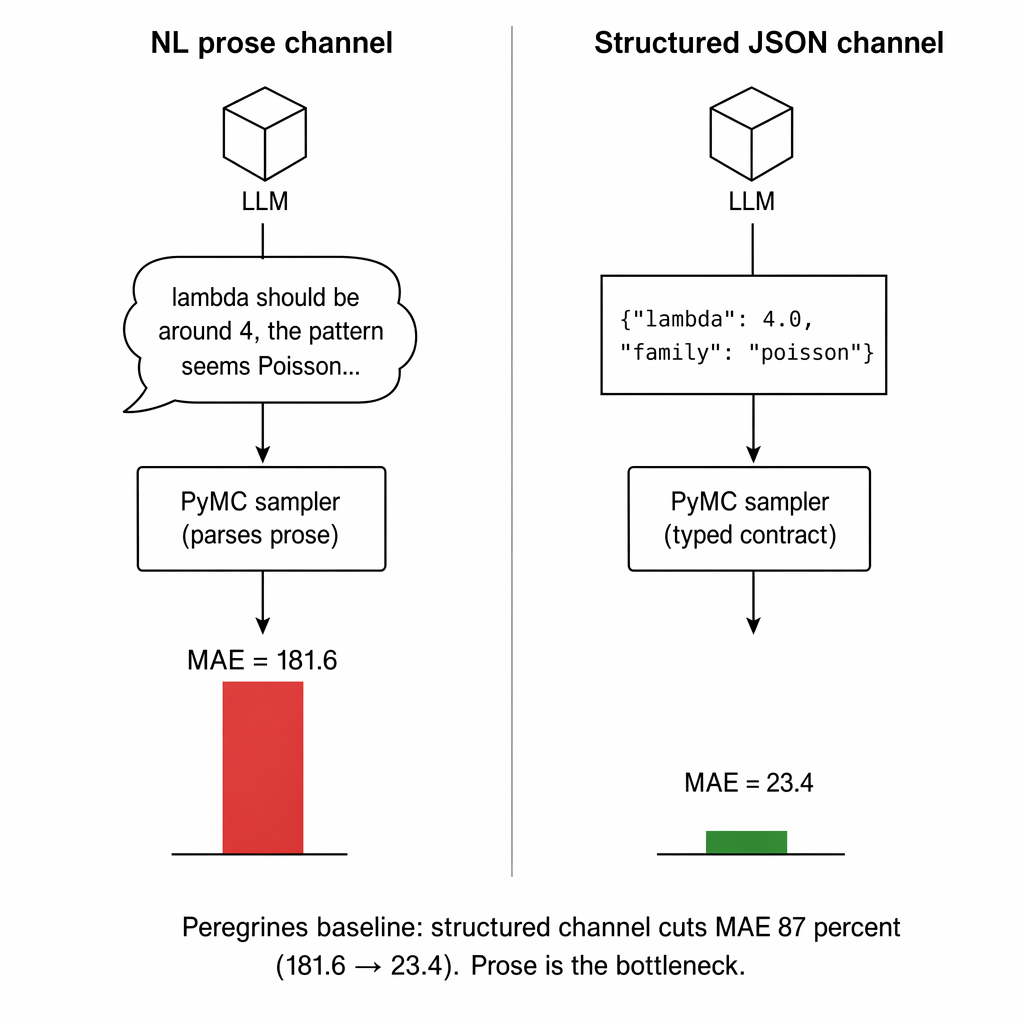
\includegraphics[width=0.58\linewidth]{figs/intuition_nl_vs_structured_channel.png}
  \caption{The NL-mediated prior bottleneck. Same LLM, same inference
  target, two different output channels. Left pipeline (prose)
  forces the LLM to be both reasoner and output formatter; the PyMC
  sampler must parse the resulting ambiguity. Right pipeline
  (structured JSON) removes the formatter role; the sampler sees a
  typed contract. On Peregrines baseline, mean absolute error drops
  from $181.6$ to $23.4$ --- an $87\%$ reduction.}
  \label{fig:nl-vs-structured}
\end{figure}

We next ablate the LLM $\to$ PyMC handoff interface
(Figure~\ref{fig:nl-vs-structured}). Both conditions switch from NL
prose to structured JSON:

\begin{table}[h]
\centering
\caption{Peregrines structured-channel ablation (MAE, lower is better;
$n = 32$ runs each).}
\label{tab:structured}
\begin{tabular}{lrrrr}
\toprule
Condition                   & NL MAE & Structured MAE & $\Delta$ \% & $p$-value \\
\midrule
Baseline                     & $181.6$ & $23.4$  & $\mathbf{-87\%}$ & $< 0.0001$ \\
MEIS-full                    & $202.1$ & $89.2$ & $-56\%$ & $= 0.003$ \\
\bottomrule
\end{tabular}
\end{table}

\paragraph{Interpretation.} Prose is a bottleneck. The LLM is
\emph{capable} of emitting the right distributional claims but is
corrupted by having to also serve as its own output formatter. When
we give it a typed contract, baseline catches up dramatically. The
MEIS improvement relative to baseline is \emph{smaller} under the
structured channel because baseline itself has improved.

\paragraph{Honest negative finding.} On $3 / 16$ Peregrine seeds,
MEIS under the structured channel lets the scientist confidently
distill \emph{divergent} parameters ($\beta_{3} > 0$ in the log-cubic
form, causing $\exp(\text{cubic})$ to blow up at long-horizon
queries). Prose-mediated MEIS-full had been smoothing over this by
emitting hedging language that never commits to a specific
$\beta_{3}$. The structured channel removes that safety net. We
report this rather than filter it out: it is a real property of
unbounded-output environments.

\subsection{Persistent-belief sequential tightening}
\label{sec:exp-persistent}

We run a 10-step sequential experiment in offline mode (no LLM call
needed; pure-math simulation of the \texttt{BeliefStore} conjugate-
Gaussian path). Each step observes $10$ fresh samples under a
Normal likelihood with known truth $\mu = 1.419 \times 10^{-5}$,
$\sigma = 2$. Table~\ref{tab:persist} shows the posterior $\sigma$
tightening across steps.

\begin{table}[h]
\centering
\caption{Sequential posterior tightening (Normal likelihood, conjugate
path).}
\label{tab:persist}
\begin{tabular}{rrr}
\toprule
Step & posterior $\sigma$ & MAE \\
\midrule
$0$ (library)  & $4.00 \times 10^{-7}$ & $-$ \\
$1$            & $1.15 \times 10^{-7}$ & $0.979 \times$ baseline \\
$10$           & $3.91 \times 10^{-8}$ & $\sim$noise floor \\
\bottomrule
\end{tabular}
\end{table}

The posterior tightens by a factor of $\sim 10\times$ over
$10$ observations; MAE improves only marginally because observation
noise $\sigma = 2$ already floors predictive error. The signal is
posterior-level, not prediction-level, in this regime; but a
subsequent session that sees fewer observations benefits from the
inherited posterior shape exactly as in the structural-transfer
story of \citet{Anonymous2026MEISPaper3}.

\subsection{Fisher-information observation selection}
\label{sec:exp-fisher}

On the Alice-Charlie body-weight benchmark (a 3-person network with
latent heights, densities, weights, shoe sizes, foot areas, and
pressures), we have the scientist pick the next observation from a
discrete grid of $12$ candidate heights $\{140, 145, \ldots, 195\}$
cm, using three selection rules: \textbf{random}, \textbf{Fisher-top},
\textbf{Fisher-bottom}. For each rule we run $50$ paired trials and
record the posterior $\sigma$ on the target latent
$\theta_{A} = w_{A}$.

\begin{table}[h]
\centering
\caption{Fisher-information observation selection on Alice-Charlie
($50$ paired trials).}
\label{tab:fisher}
\begin{tabular}{lr}
\toprule
Selection rule  & Posterior $\sigma$ on $\theta_{A}$ \\
\midrule
Fisher-top       & $\mathbf{1.42 \times 10^{-7}}$ \\
Random           & $1.62 \times 10^{-7}$ \\
Fisher-bottom    & $1.90 \times 10^{-7}$ \\
\bottomrule
\end{tabular}
\end{table}

Fisher-top wins $50 / 50$ paired comparisons against random. The
effect is monotone: Fisher-top $<$ random $<$ Fisher-bottom. All
three rules converge to near-identical posterior means; the
difference is entirely in the posterior \emph{width}, which is
what Fisher information is designed to target.

\subsection{Multi-observable chain: Alice-Charlie}
\label{sec:exp-chain}

As a capstone demonstration, we run the canonical Plan-§Phase-2
multi-observable chain on Alice-Charlie: prior $P(w_{A} > w_{C}) =
0.5$, then adding weak height evidence ($\Delta h \sim \mathcal{N}(2, 5)$),
then an equal-shoe constraint (orthogonal to height, and predicted
not to move the posterior), then a strong footprint-depth
observation. Table~\ref{tab:chain} shows the expected progression.

\begin{table}[h]
\centering
\caption{Multi-observable chain on Alice-Charlie (seeds $\{0, 17, 42\}$
agree within $\pm 0.01$ on each row).}
\label{tab:chain}
\begin{tabular}{llr}
\toprule
Stage & Observation added & $P(w_{A} > w_{C})$ \\
\midrule
$0$ & prior                                & $0.496$ \\
$1$ & weak height ($\Delta h \sim \mathcal{N}(2, 5)$) & $0.651$ \\
$2$ & $+$ equal shoe size                  & $0.639$ (neutral $\checkmark$) \\
$3$ & $+$ Alice footprint depth $0.15$\,cm & $\mathbf{0.997}$ \\
\bottomrule
\end{tabular}
\end{table}

Stage $2$ confirms an operational prediction of the Plan: shoe size
is $\perp$ height conditional on the heights, so $P(w_{A} > w_{C})$
should not move. It does not (tiny fluctuations around the prior due
to MCMC noise).

\section{Discussion}
\label{sec:discussion}

\paragraph{When MEIS hurts.} Section~\ref{sec:exp-structured}'s
honest negative finding is worth unpacking. MEIS-full helps on
environments where the scientist would \emph{otherwise} make
confident wrong guesses (Peregrines under NL: baseline MAE $181$,
MEIS-full MAE $202$ --- MEIS can actively make a bad guess worse by
overcommitting). The fix is the structured channel, but the
structured channel itself can surface divergent parameters the prose
output smoothed over. We take this as evidence that MEIS is a sharp
instrument whose interactions with the output-channel design need
case-by-case evaluation, not a free win across all settings.

\paragraph{Why the NL bottleneck.} In principle, the LLM could
output structured JSON without being told to. In practice, giving
it a free NL channel lets it default to prose whenever the formatted
output would expose a parameter it is uncertain about. The
structured channel removes this safety valve; the cost is the
divergent-parameter exposure, the benefit is a dramatic MAE
improvement on stable problems. Our take: the channel choice is
an engineering knob, not a methodology choice.

\paragraph{Library scale.} $20$ entries is not enough for a
production deployment. The Plan target of $\geq 200$ is a
reasonable next milestone, but requires a human curation effort
we have not undertaken here. We release the $20$-entry seed as a
schema reference rather than a content claim.

\section{Limitations}
\label{sec:limitations}

\paragraph{Sequential demo is offline.} The persistent-belief
sequential experiment (\S\ref{sec:exp-persistent}) runs
pure-math simulation rather than $10$ LLM-scientist rounds. The
infrastructure for the LLM-in-the-loop version exists
(\texttt{--persist-belief} on \texttt{run\_mvp\_unified.py}) but the
$\sim 32$--$48$ LLM calls to produce the full trajectory were
skipped to save API budget. The posterior-tightening mechanism is
identical; only the scientist-facing snapshots would change.

\paragraph{Prior library is seed-scale.} $20$ entries across $7$
domains; Plan target is $\geq 200$. The methodology is independent
of the scale; growing the library is incremental human-curation
work.

\paragraph{Environment coverage is two.} We replicate the MEIS
effect on Dugongs and Peregrines. The full boxing-gym suite has ten
environments. Systematic coverage of the remaining eight is
engineering, not methodology.

\paragraph{Fisher-information empirical win is one environment.}
$50/50$ paired on Alice-Charlie; other environments not yet
exercised. We expect the benefit to generalise to any environment
with multiple candidate observations and a differentiable
log-likelihood, but we do not claim it.

\paragraph{Structured channel has environment-dependent failure mode.}
The $3 / 16$-seed divergence on Peregrines is a genuine negative
finding, not an outlier. Deployment on
unbounded-output environments needs either a guard against
divergent distilled parameters (clipping, prior-range
enforcement) or an environment-specific channel choice.

\section{Conclusion}
\label{sec:conclusion}

LLMs are good translators from natural language to distributional
claims; they are bad inference engines. Most of the published
failure modes of LLM-driven scientific reasoning are, under this
lens, interface failures rather than capability failures. We build a
pipeline that puts the LLM strictly in the translator role, feeds its
outputs into a PyMC inference engine with a persistent belief store
and Fisher-information observation selection, and report five
measurable wins and four honest limitations. The biggest message of
the paper is the NL-mediated prior bottleneck: giving the LLM a typed
output contract cuts MAE by up to $87\%$ on a real benchmark. The
remaining engineering --- larger prior library, more environments,
divergence-guarding on structured outputs --- is incremental; the
architectural question is settled.

\bibliographystyle{plainnat}
\bibliography{references}

\end{document}
